%!TEX root = thesis.tex

\chapter{Research Design}
\label{chp:Research_Design}

This chapter outlines the research methodology employed in this study. It details the rationale behind the research questions, the chosen methodological approach, and the procedures for data collection and analysis. Section~\ref{sec:ResearchMethodologyApproach} first introduces the overarching methodological framework guiding this research. Subsequently, Section~\ref{sec:ResearchObjectivesAndQuestions} systematically defines the study’s objectives and research questions, forming the foundation for subsequent analyses. Section~\ref{sec:LiteratureReviewProcess} then discusses the literature review methodology, which primarily involved a \gls{sms} complemented by elements of a \gls{slr}, incorporating search strategies, selection criteria, and data synthesis. Finally, Section~\ref{sec:FrameworkEvaluationMethodology} describes the case study approach used for the empirical evaluation of the proposed framework.

~\\
\vfill
\minitoc
\clearpage

\section{Methodological Approach}
\label{sec:ResearchMethodologyApproach}

The current study adopts the \gls{dsr} methodology as outlined by Vom Brocke et al. \cite{vombrockeIntroductionDesignScience2020} and Peffers et al. \cite{peffersDesignScienceResearch2012}. \Gls{dsr} offers a structured yet flexible framework for integrating multiple research methods, rendering it well-suited for the mixed-methods approach of this research. A core component of the \gls{dsr} process involved a comprehensive literature analysis to establish a robust theoretical foundation for the framework design. This analysis began with a systematic search and snowballing process to gather a relevant set of publications.

The identified corpus of literature then served as the basis for two complementary analytical stages. First, to systematically map the research landscape and identify broader trends and gaps, a \gls{sms} was conducted following the guidelines of Petersen et al. \cite{petersenGuidelinesConductingSystematic2015}. The \gls{sms} facilitated a structured categorization and quantification of contributions, offering a wide perspective on existing work and underexplored areas.

Second, to gain deeper insights from the most pertinent studies within this corpus, elements of a \gls{slr} were incorporated. This involved applying principles from Kitchenham and Charters \cite{kitchenhamGuidelinesPerformingSystematic2007} for more detailed data extraction from selected papers. Such a combined approach, emphasizing the breadth of an \gls{sms} while integrating the depth of focused \gls{slr} techniques on the same initial paper set, aimed to ensure both a comprehensive overview and a nuanced understanding of critical contributions informing the framework development.

Subsequently, an empirical case study was conducted to validate the practical applicability of the proposed framework within a simulated real-world scenario. This validation step helps to ensure that the framework is not only theoretically grounded but also practically relevant. Figure~\ref{fig:research-methodology} provides a visual representation of the overall \gls{dsr} process applied.

\begin{figure}[htbp]
    \centering
    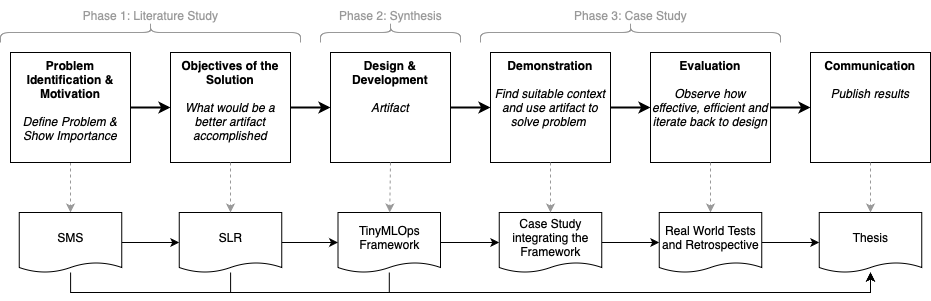
\includegraphics[width=0.975\textwidth]{figs/research_design/dsr-diagramm.png}
    \caption[Research Methodology Overview]{Overview of the Design Science Research approach applied in this study.}
    \label{fig:research-methodology}
\end{figure}

\section{Research Objectives and Questions}
\label{sec:ResearchObjectivesAndQuestions} 

The \glspl{rq} are addressed through a structured methodological approach. Each research phase is designed to progressively refine the understanding of \gls{tinymlops} requirements, best practices, and implementation challenges. RQ1 and RQ2 are primarily addressed through the \gls{sms} and the supplementary \gls{slr} findings. RQ3 is tackled by the conceptual framework design, informed by these literature analyses. Finally, RQ4 is investigated through the case study evaluation of the developed framework. The study is structured around the following \glspl{rq}:

\begin{tabularx}{\textwidth}{@{}lX@{}}
    \textbf{RQ1:} & \emph{What system architectures, methodologies, and practices are employed to support \gls{tinyml} in resource-constrained embedded systems?} \\  
                  & This question examines the current landscape of \gls{tinyml} deployments, analyzing architectural patterns, and design strategies in embedded environments. \\[0.5em]

    \textbf{RQ2:} & \emph{Which frameworks and strategies facilitate decentralized on-device \gls{mlops} while minimizing reliance on cloud infrastructure?} \\  
                  & This question explores methodologies for continuous on-device learning, model retraining, and monitoring in decentralized systems, identifying \gls{lcm} techniques that reduce dependency on cloud-based resources. \\[0.5em]

    \textbf{RQ3:} & \emph{How can a \gls{tinymlops} framework be designed to enable effective on-device model \gls{lcm} in resource-constrained systems?} \\  
                  & Building upon insights from RQ1 and RQ2, this question focuses on the development of a \gls{tinymlops} framework, integrating key methodologies to support model deployment, adaptation, and \gls{lcm}. \\[0.5em]

    \textbf{RQ4:} & \emph{How does deploying on-device TinyMLOps in decentralized embedded systems influence deployment complexity, resource consumption, and performance trade-offs?} \\  
                  & This question shifts the focus from theoretical design to empirical validation, assessing the feasibility of the proposed framework through a case study. It examines deployment complexities, performance trade-offs, and practical constraints that impact real-world implementations. \\  
\end{tabularx}


\section{Literature Analysis Process}
\label{sec:LiteratureReviewProcess}

The literature analysis process commenced with an exploratory search in Google Scholar, employing a broad approach to scan a wide range of publications. This initial step aimed to establish a foundational understanding of key terminologies, emerging research trends, and thematic patterns within \gls{tinymlops} and resource-constrained on-device \gls{ml}. During this phase, three particularly relevant studies were identified. These served as seed papers to refine the research focus and provided key insights that contributed to formulating the initial \glspl{rq} and defining inclusion and exclusion criteria for the subsequent systematic search. Figure~\ref{fig:slr-process} provides an overview of this multi-stage process, outlining the key methodological steps.

\begin{figure}[htbp]
    \centering
    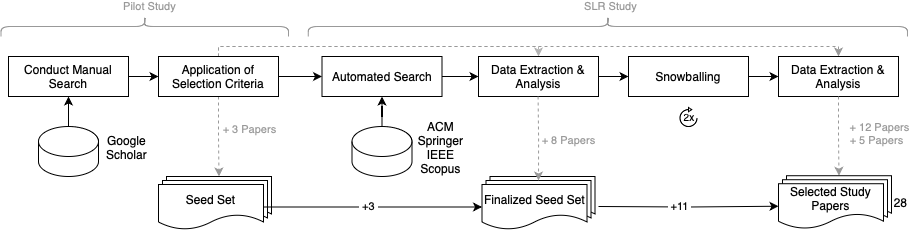
\includegraphics[width=0.975\textwidth]{figs/research_design/SLR-diagramm.png}
    \caption[Systematic Literature Review Process Overview]{Overview of the Systematic Literature Review Process applied in this study.}
    \label{fig:slr-process}
\end{figure}

\subsection{Data Collection}
\label{ssec:data_collection}

While the initial pilot study exclusively relied on Google Scholar, the subsequent systematic search targeted four major literature indexing platforms: ACM Digital Library, SpringerLink, IEEE Xplore, and Scopus. The search strategy was designed to prioritize precision over recall. Such a focus ensured that primarily studies directly relevant to \gls{tinymlops} were included, thereby minimizing the inclusion of irrelevant publications. The final query formulation incorporated key terms such as ``MLOps'' and ``Embedded Machine Learning,'' as detailed in table~\ref{tab:tinymlops-query}.

\begin{table}[htbp]
 \caption[Search Query Structure for TinyMLOps Literature]{Search Query Structure for TinyMLOps Literature.}
\label{tab:tinymlops-query}
\begin{tabularx}{\linewidth}{@{}lL@{}}
\opentableheader
\hl{Query Element} & \hl{Search Terms} \\
\closetableheader
TinyML Domain & ``TinyML'' OR ``Tiny Machine Learning'' OR ``Embedded Machine Learning'' OR ``On-device Machine Learning'' \\
MLOps Domain & ``MLOps'' OR ``Machine Learning Operations'' OR ``Lifecycle Management'' OR ``Operationalization'' OR ``Continuous Training'' OR ``Model Monitoring'' OR ``TinyMLOps'' \\
\bottomrule
\end{tabularx}
\end{table}


\subsection{Application of Selection Criteria}
\label{ssec:selection_criteria}

Following the identification of potentially relevant studies, a manual selection process was conducted based on the inclusion and exclusion criteria. A study was confirmed as a primary source if it satisfied all inclusion criteria and did not meet any exclusion criteria. The selection criteria are detailed in table~\ref{tab:criteria}.

\begin{table}[htbp]
    \caption[Inclusion and Exclusion Criteria for the SLR]{Inclusion and Exclusion Criteria for the Systematic Literature Review.}
    \label{tab:criteria}
    \begin{tabularx}{\linewidth}{@{}lX@{}}
        \opentableheader
        \hl{Criteria Type} & \hl{Description} \\
        \closetableheader
        IC1                & The study addresses \gls{tinyml} concepts, methodologies, or challenges. \\
        IC2                & The study presents practical implementations, experiments, or real-world case studies in the \gls{tinyml} domain, relevant for operations of models. \\
        IC3                & The study addresses lifecycle management characteristics of \gls{ai}-based applications on embedded devices. \\
        \midrule
        EC1                & The study does not meet basic scientific standards (e.g., clear methodology, reproducibility, logical reasoning in conclusions). \\
        EC2                & The study has not undergone peer review or appears in non-reputable sources. \\
        EC3                & The study does not contribute original research or data (e.g., meta-analyses, secondary reviews, purely conceptual discussions without validation). \\
        EC4                & The study was published before 2020. \\
        \bottomrule
    \end{tabularx}
\end{table}

\subsection{Snowballing}
\label{ssec:snowballing}

To enhance the comprehensiveness of the literature mapping and mitigate potential gaps in the automated search results, a bidirectional snowballing process was conducted following Wohlin’s guidelines \cite{wohlinGuidelinesSnowballingSystematic2014a}. This procedure involved both backward snowballing (identifying references cited in selected papers) and forward snowballing (identifying studies that cited the selected papers). Starting with an initial seed set of 11 papers, two iterative rounds of backward and forward snowballing were performed. These iterations led to the inclusion of 17 additional studies after full-text screening. This snowballing process continued until no further relevant studies were identified.

\subsection{Data Extraction}
\label{ssec:data_extraction}

A structured data extraction process was implemented to ensure consistency and traceability across all reviewed studies. For this purpose, a custom extraction template was designed to capture key aspects of the literature. Such aspects were subsequently categorized into five primary dimensions, as detailed in table~\ref{tab:data_extraction_dimensions}.

\begin{table}[htbp]
    \caption[Primary Data Extraction Dimensions]{Primary Data Extraction Dimensions for Literature Analysis.}
    \label{tab:data_extraction_dimensions}
    \begin{tabularx}{\linewidth}{@{}lX@{}}
        \opentableheader
        \hl{Dimension} & \hl{Description} \\
        \closetableheader
        Research Context                & Defines the study’s objective, scope, and classification. \\
        MLOps and Architectural Approaches & Identifies architectural frameworks, \gls{mlops} methodologies, network constraints, and applied technologies. \\
        Hardware and ML Algorithms      & Categorizes hardware platforms and \gls{ml} algorithms used for on-device learning. \\
        Case Studies and Results        & Extracts empirical evidence from real-world deployments or experimental implementations. \\
        Identified Research Gaps        & Assesses limitations discussed, scientific quality considerations, and stated future research directions. \\
        \bottomrule
    \end{tabularx}
\end{table}

To capture characteristics specifically relevant to \gls{tinymlops}, six additional subcategories were defined within the broader dimensions, primarily under ``MLOps and Architectural Approaches'' and ``Hardware and AI Use Case''. The subcategories, listed in table~\ref{tab:tinymlops_subcategories}, facilitated a more granular analysis of the \gls{tinymlops} domain.

\begin{table}[htbp]
    \caption[TinyMLOps-Specific Data Extraction Subcategories]{TinyMLOps-Specific Data Extraction Subcategories.}
    \label{tab:tinymlops_subcategories}
    \begin{tabularx}{\linewidth}{@{}lX@{}}
        \opentableheader
        \hl{Subcategory} & \hl{Description} \\
        \closetableheader
        System Architecture             & Describes the overall system design, including architectural patterns and system behavior. \\
        Runtime Characteristics         & Clusters the runtime environment employed (e.g., compiled, interpreter-based). \\
        Model Training and Optimization & Covers training methodologies (e.g., central, decentralized, hybrid) and model optimization techniques. \\
        Model Management                & Details concepts and practices used for model \gls{lcm} (e.g., versioning, deployment strategies). \\
        CI/CD Practices                 & Clusters automation strategies observed for continuous integration and continuous deployment in the context of \gls{tinyml}. \\
        Monitoring Aspects              & Investigates metrics and strategies utilized for continuous monitoring of models and systems. \\
        \bottomrule
    \end{tabularx}
\end{table}

\subsection{Data Synthesis}
\label{subsec:DataSynthesis}

Following data extraction, a structured synthesis was performed to identify key research trends, technological patterns, and knowledge gaps within \gls{tinymlops}. This synthesis process combined classification techniques, structured mappings, and visual analytics to ensure a comprehensive evaluation of the research landscape. Selected studies were categorized according to research type and contribution type. For research type classification, the method by Wieringa et al. \cite{wieringaRequirementsEngineeringPaper2006} was adopted, distinguishing between solution proposals, validation studies, evaluation studies, philosophical discussions, and experience reports. In parallel, contribution type classification categorized studies based on their outputs, such as frameworks, tools, models, or conceptual insights.

A key component of the synthesis involved mapping \gls{tinymlops} methodologies against hardware constraints. Given the computational limitations of embedded systems, a classification framework was introduced that categorizes hardware based on processing power, memory capacity, and energy efficiency. To further visualize relationships between research domains, methodologies, and technological constraints, multiple mapping studies were conducted employing bubble charts and co-occurrence matrices. Such visualizations enabled a clearer identification of concentrated research areas, emerging trends, and underexplored gaps.

\section{Framework Evaluation Methodology}
\label{sec:FrameworkEvaluationMethodology}

The empirical evaluation of the proposed \gls{tinylcm} framework follows the structured approach outlined by Wohlin et al. \cite{wohlinExperimentationSoftwareEngineering2024}. This methodology ensures a systematic assessment of the framework's feasibility, performance characteristics, and operational constraints under resource-constrained conditions. The evaluation design evolved through iterative refinement, beginning with an ambitious field deployment protocol and culminating in a controlled quasi-experiment that better isolates the framework's core capabilities while maintaining practical relevance.

\subsection{Evolution of the Experimental Design}
\label{ssec:experimental_design_evolution}

Initial planning for the evaluation of \gls{tinylcm} envisioned a series of experiments directly deploying the framework on a battery-powered, mobile Mars rover prototype (a 4tronix kit\footnote{The specific kit used is the 4tronix Mars Rover Robot Kit, further details available at: \url{https://www.elektor.de/products/4tronix-mars-rover-robot-kit-for-raspberry-pi-zero}.} equipped with a Raspberry Pi Zero 2W). The goal was to assess performance, including drift detection, under dynamic conditions across several scenarios involving different object classes and novel ``drift'' objects. However, experiments on this setup revealed significant practical challenges that confounded the ability to isolate and reliably measure the framework's specific contributions:

\begin{itemize}[noitemsep, topsep=0pt]
    \item \textit{Power Instability:} The battery power (four AA alkaline batteries) proved insufficient for sustained operation during computationally intensive phases (camera capture, \gls{tfl} inference, feature processing, and drift monitoring), leading to frequent system shutdowns.
    \item \textit{Hardware Configuration Discrepancies:} Unforeseen differences between the development camera (Pi Camera V2) and the rover's camera (Pi Camera V1.3) introduced variability in image quality and characteristics, impacting model performance.
    \item \textit{Environmental Variability:} Uncontrolled lighting, reflections, and inconsistent object positioning relative to the camera created excessive noise in the data, making it difficult to distinguish genuine concept drift from environmental fluctuations.
    \item \textit{Base Model Performance:} The classification model's accuracy was sometimes insufficient. Misclassifications were potentially misinterpreted as known objects, thus complicating the evaluation of the drift detection mechanisms themselves. This was influenced by both suboptimal model training and environmental variability.
    \item \textit{Timing Mismatch and Data Interpretation:} The experiment initially used a standard system configuration for inference (five frames per second). With objects presented for only two seconds, this led to difficulties in data interpretation, further complicated by the model performance issues, making it hard to determine exact causalities.
    \item \textit{Connectivity and Data Collection Issues:} Unstable SSH connections, due to an unstable network in the laboratory on those days, hindered real-time monitoring and reliable data acquisition during remote rover operation.
\end{itemize}

These limitations underscored the difficulty of conducting rigorous, reproducible experiments in uncontrolled embedded systems. The key lesson learned was the necessity for a more controlled experimental setup to isolate the framework's performance and systematically validate its core functionalities before tackling the full complexity of a dynamic field deployment. This led to the development of a refined experimental design, focusing on controlled laboratory assessments.

\subsection{Experimental Design}
\label{ssec:refined_experimental_design_final}

The refined experimental design aims to systematically evaluate \gls{tinylcm}'s capabilities concerning performance overhead, functional drift detection, and operational robustness on a stationary Raspberry Pi Zero 2W platform. This approach directly supports the investigation of RQ4.

\paragraph{Evaluation Objectives}
The core objectives are to:
\begin{enumerate}[noitemsep, topsep=0pt]
    \item Quantify the computational and memory overhead introduced by \gls{tinylcm}'s components.
    \item Validate the framework's on-device, unsupervised drift detection capabilities under controlled conditions.
    \item Assess system stability and resource utilization during extended operation.
\end{enumerate}

\paragraph{Experiment Hypotheses}
These objectives are translated into the following testable hypotheses:

\begin{tabularx}{\textwidth}{@{}lX@{}}
    \textbf{H$_1$:} & \textit{Performance Overhead:} The computational overhead from \gls{tinylcm} components  increases inference latency by less than 50\% compared to baseline \gls{tfl} inference. This threshold is chosen to ensure that real-time performance, critical for many edge applications, is maintained. \\[0.5em]

    \textbf{H$_2$:} & \textit{Resource Constraints:} The complete \gls{tinylcm} framework operates within defined resource bounds on the target hardware, maintaining average CPU utilization below 50\% (allowing headroom for other system tasks) and memory consumption below \SI{256}{\mega\byte} of the \SI{512}{\mega\byte} available. \\[0.5em]

    \textbf{H$_3$:} & \textit{Drift Detection:} The alarm rate generated by the \gls{tinylcm} framework during periods where untrained (drift) objects are presented is statistically significantly higher than the alarm rate during periods with known objects or background samples. \\
\end{tabularx}

\paragraph{Experimental Setup and Configuration}
All refined quasi-experiments are conducted on a Raspberry Pi Zero 2W, serving as a representative demonstration of a resource-constrained \glspl{sbc}. The key components and configurations of the experimental setup are summarized in Table~\ref{tab:experimental_setup_config}.

\begin{table}[htbp]
    \caption[Refined Experimental Setup and Configuration Details]{Detailed Configuration of the Refined Experimental Setup.}
    \label{tab:experimental_setup_config}
    \begin{tabularx}{\linewidth}{@{}lX@{}} 
        \toprule
        \textbf{Component/Aspect} & \textbf{Specification / Configuration} \\
        \midrule
        Target Hardware & Raspberry Pi Zero 2W \\
        & \textit{SoC:} Broadcom BCM2710A1 (\SI{1}{\giga\hertz} quad-core ARM Cortex-A53) \\
        & \textit{Memory:} \SI{512}{\si{\mega\byte}} LPDDR2 SDRAM \\
        & \textit{Storage:} \SI{32}{\si{\giga\byte}} microSD card \\
        & \textit{Camera:} Raspberry Pi Camera Module V2 (8-megapixel sensor) \\
        \addlinespace 
        Operating System & Raspberry Pi OS Lite (32-bit) \\
        & \textit{Base:} Debian version 12 ``bookworm'' \\
        \addlinespace
        ML Model & MobileNetV2, INT8 quantized (\gls{tfl}) \\ 
        & \textit{Training Data Classes:} ``lego'', ``stone'', ``leaf'', ``negative''. \\
        & \textit{Feature Processing:} L2 Normalization, PCA (1280-D $\rightarrow$ 256-D). \\
        \bottomrule
    \end{tabularx}
\end{table}

The experimental environment is further controlled for lighting (dual artificial sources, no direct sunlight), camera position (fixed at \SI{15}{\centi\meter} from objects), and object placement (defined markings) to ensure consistency across all trials.

\paragraph{Experimental Phases and Scenarios}
The evaluation comprises two main phases:

\textit{Phase 1: Performance Overhead Assessment.} This phase quantifies the computational and memory overhead of \gls{tinylcm} components. It utilizes the three staged configurations previously described: (i) Baseline (\gls{tfl} inference only), (ii) Enhanced Pipeline (\gls{tfl} with feature processing and \gls{knn} classification), and (iii) Complete Framework (full \gls{tinylcm} with drift monitoring).
Each of these three configurations will be executed in five independent runs to account for system variability and enable robust statistical comparisons. Each run will last for a total of \SI{150}{\second}, performing inferences at a rate of five frames per second. The sequence within each run is structured as follows:
\begin{itemize}[noitemsep, topsep=0pt, leftmargin=1em]
    \item \textit{0-30 seconds:} Warm-up period presenting ``negative'' (background) samples. Data from this period will be excluded from performance analysis.
    \item \textit{30-60 seconds:} Presentation of a known object (``lego'').
    \item \textit{60-90 seconds:} Presentation of ``negative'' (background) samples.
    \item \textit{90-120 seconds:} Presentation of a ``drift'' object (``ball'').
    \item \textit{120-150 seconds:} Presentation of ``negative'' (background) samples.
\end{itemize}
Performance metrics (CPU usage, memory consumption, inference latency) will be collected throughout the \SI{120}{\second} following the warm-up period (from seconds 31--150). This phase primarily targets hypotheses H$_1$ and H$_2$.

\textit{Phase 2: Drift Detection Validation.} This phase validates functional drift detection (addressing H$_3$) using two scenarios (Table~\ref{tab:drift_scenarios_refined}) with a reduced frame rate. Known objects are presented for approx. \SI{10}{\second} (5 frames), drift objects for \SI{30}{\second}.

\begin{table}[htbp]
  \caption[Drift Detection Scenarios]{Phase 2 Drift Detection Scenarios (1 inference per 2 seconds).}
  \label{tab:drift_scenarios_refined}
  \begin{tabularx}{\linewidth}{@{}lX@{}}
    \toprule 
    \textbf{Scenario ID} & \textbf{Specification} \\ 
    \midrule 
    S1: Dual Drift & 
      \textit{Trained classes:} ``negative'', ``lego'', ``leaf'', ``stone''. \newline
      \textit{Drift objects (untrained):} ``coin'', ``ball''. \newline
      \textit{Sequence:} neg $\rightarrow$ leaf $\rightarrow$ stone $\rightarrow$ neg $\rightarrow$ lego $\rightarrow$ neg $\rightarrow$ \textbf{ball} $\rightarrow$ neg $\rightarrow$ \textbf{coin} $\rightarrow$ neg $\rightarrow$ lego $\rightarrow$ neg. \\[0.5em]

    S2: Single Drift & 
      \textit{Trained classes:} ``negative'', ``lego'', ``leaf'', ``stone'', ``coin''. \newline
      \textit{Drift object (untrained):} ``ball''. \newline
      \textit{Sequence:} neg $\rightarrow$ leaf $\rightarrow$ stone $\rightarrow$ neg $\rightarrow$ lego $\rightarrow$ neg $\rightarrow$ coin $\rightarrow$ neg $\rightarrow$ \textbf{ball} $\rightarrow$ neg $\rightarrow$ lego $\rightarrow$ neg. \\
    \bottomrule
  \end{tabularx}
\end{table}

\paragraph{Data Collection, Metrics, and Analysis Plan}
Data collection includes automated logging of performance metrics (inference latency, CPU utilization, memory usage) and functional metrics (drift alarm timestamps, confidence scores). Descriptive statistics will characterize the performance. Statistical analyses will be performed using Python with libraries such as SciPy and statsmodels: 

For key quantitative metrics (latency, \gls{cpu} usage, memory usage) derived from the $n=5$ independent runs per configuration, the normality of their distributions will be assessed using the Shapiro-Wilk test \cite{shapiroAnalysisVarianceTest}. The choice between parametric tests (t-tests) and their appropriate non-parametric counterparts will be based on this assessment. A significance level of $\alpha = 0.05$ will be used for all hypothesis testing.

\paragraph{Hypothesis Testing for Performance (H$_1$ and H$_2$)}
The evaluation of performance overhead (H$_1$) and resource constraints (H$_2$) follows the structured plan detailed in Table~\ref{tab:analysis_plan_h1_h2}. The table outlines the specific metrics, statistical tests, and effect size measures used to compare the observed performance against the defined thresholds and to compare the different experimental configurations against each other.

\begin{table}[htbp]
    \caption{Analysis Plan for Performance Hypotheses H$_1$ and H$_2$.}
    \label{tab:analysis_plan_h1_h2}
    \begin{tabularx}{\linewidth}{@{}>{\raggedright\arraybackslash}p{0.07\textwidth} >{\raggedright\arraybackslash}p{0.21\textwidth} >{\raggedright\arraybackslash}X >{\raggedright\arraybackslash}p{0.3\textwidth}@{}}
        \toprule
        \textbf{Hypo\-thesis} & \textbf{Evaluation Metric} & \textbf{Statistical Test} & \textbf{Effect Size Measures} \\
        \midrule
        \textbf{H$_1$} & Inference latency relative to baseline.
        
        \textit{Threshold: < 50\%} & 
        \textit{One-sided one-sample t-test} (if normal) or \textit{one-sided Wilcoxon signed-rank test} (if not normal) to test against the 50\% threshold. &
        The test will be performed on the distribution of latency increases for each configuration. \\
        \addlinespace
        \textbf{H$_2$} & CPU usage. 
        
        \textit{Threshold: < 50\%} & 
        \textit{One-sided one-sample t-test} (if normal) or \textit{one-sided Wilcoxon signed-rank test} (if not normal) to test the distribution of CPU values against the 50\% threshold. & 
        For comparing configurations, \textit{Welch's t-test} or the \textit{Mann-Whitney U test} will be used. Effect size will be quantified using \textit{Cohen's d} or \textit{Cliff's delta}, respectively. \\
        \addlinespace
        \textbf{H$_2$} & Memory consumption. 
        
        \textit{Threshold: < 256 MB} & 
        \textit{One-sided one-sample t-test} (if normal) or \textit{one-sided Wilcoxon signed-rank test} (if not normal) to test the distribution of memory values against the 256 MB threshold. &
        The hypothesis is primarily supported if all values are below the threshold. The statistical test provides additional formal evidence. \\
        \bottomrule
    \end{tabularx}
\end{table}

\paragraph{Hypothesis Testing for Drift Detection (H$_3$)}
The evaluation of drift detection (H$_3$) focuses on assessing the statistical significance of the detection mechanism. The analysis plan, detailed in Table~\ref{tab:analysis_plan_h3}, is designed to determine whether the framework's response to untrained objects is a reliable, non-random event.

\begin{table}[htbp]
    \caption{Analysis Plan for Drift Detection Hypothesis H$_3$.}
    \label{tab:analysis_plan_h3}
    \begin{tabularx}{\linewidth}{@{}>{\raggedright\arraybackslash}p{0.14\textwidth} >{\raggedright\arraybackslash}X >{\raggedright\arraybackslash}p{0.34\textwidth}@{}}
        \toprule
        \textbf{Hypothesis} & \textbf{Metric and Test Condition} & \textbf{Primary Statistical Test and Method} \\
        \midrule
        \textbf{H$_3$} & 
        \textit{Metric:} Proportion of drift alarms.
        
        \textit{Condition:} The alarm rate during ``drift periods'' must be significantly higher than during ``non-drift periods'' ($p < 0.05$). &
        A 2x2 contingency table (Period Type vs. Alarm Triggered) will be created. 
        
        \textit{Fisher's Exact Test} will be used to test for a significant association. \\
        \bottomrule
    \end{tabularx}
\end{table}

\subsection{Threats to Validity}
\label{ssec:evaluation_threats_to_validity}

The refined experimental design aims to mitigate several threats to validity, though some limitations, summarized in Table~\ref{tab:threats_to_validity}, remain.

\begin{table}[htbp]
    \caption[Threats to Validity and Mitigation Strategies for the Refined Experiment]{Threats to Validity and Mitigation Strategies for the Refined Experimental Design.}
    \label{tab:threats_to_validity}
    \begin{tabularx}{\linewidth}{@{}lX@{}}
        \toprule
        \textbf{Threat Category} & \textbf{Description and Mitigation/Acknowledgement} \\
        \midrule
        Internal Validity & 
        \textit{Order effects:} Minimized by consistent system initialization and controlled sequences. The reduced frame rate in Phase 2 also helps ensure consistent temporal object representation. \\
        \addlinespace
        Construct Validity & 
        \textit{Operationalization of ``drift'':} Defined as presentation of untrained object classes. While enabling controlled experiments, this may not fully represent all real-world concept drift complexities. The focus is on detecting statistical feature distribution changes. \\
        \addlinespace
        External Validity & 
        \textit{Hardware generalizability:} Results from the Raspberry Pi Zero 2W offer insights for similar \gls{sbc}s but may not directly transfer to all \gls{mcu}-based platforms or diverse application domains. \newline
        \textit{Environmental realism:} The controlled lab environment, necessary for precision, differs from dynamic field conditions encountered in the initial pilot. \\
        \addlinespace
        Statistical Validity & 
        \textit{Sample size (Phase 1):} Performance data is collected over numerous frames, allowing for robust statistical comparison. \newline
        \textit{Sample size (Phase 2):} The number of distinct drift events per scenario is limited, precluding extensive quantitative generalization of drift detection metrics; hence the focus on qualitative timeline analysis for H$_3$. Effect sizes for performance (H$_1$, H$_2$) will address practical significance beyond p-values. \\
        \bottomrule
    \end{tabularx}
\end{table}

